%%%%%%%%%%%%%%%%%%%%%%% file pepr_pub.tex %%%%%%%%%%%%%%%%%%%%%%%%%
%
%  Manuscript: PEPR: Pipeline for Evaluating Prokaryotic References
%  Authored: September 2015
%  
%%%%%%%%%%%%%%%%%%%%%%%%%%%%%%%%%%%%%%%%%%%%%%%%%%%%%%%%%%%%%%%%%%%
%\documentclass{svjour3}                     % onecolumn (standard format)
%\documentclass[smallcondensed]{svjour3}     % onecolumn (ditto)
\documentclass[smallextended]{svjour3}\usepackage[]{graphicx}\usepackage[]{color}
%% maxwidth is the original width if it is less than linewidth
%% otherwise use linewidth (to make sure the graphics do not exceed the margin)
\makeatletter
\def\maxwidth{ %
  \ifdim\Gin@nat@width>\linewidth
    \linewidth
  \else
    \Gin@nat@width
  \fi
}
\makeatother

\definecolor{fgcolor}{rgb}{0.345, 0.345, 0.345}
\newcommand{\hlnum}[1]{\textcolor[rgb]{0.686,0.059,0.569}{#1}}%
\newcommand{\hlstr}[1]{\textcolor[rgb]{0.192,0.494,0.8}{#1}}%
\newcommand{\hlcom}[1]{\textcolor[rgb]{0.678,0.584,0.686}{\textit{#1}}}%
\newcommand{\hlopt}[1]{\textcolor[rgb]{0,0,0}{#1}}%
\newcommand{\hlstd}[1]{\textcolor[rgb]{0.345,0.345,0.345}{#1}}%
\newcommand{\hlkwa}[1]{\textcolor[rgb]{0.161,0.373,0.58}{\textbf{#1}}}%
\newcommand{\hlkwb}[1]{\textcolor[rgb]{0.69,0.353,0.396}{#1}}%
\newcommand{\hlkwc}[1]{\textcolor[rgb]{0.333,0.667,0.333}{#1}}%
\newcommand{\hlkwd}[1]{\textcolor[rgb]{0.737,0.353,0.396}{\textbf{#1}}}%

\usepackage{framed}
\makeatletter
\newenvironment{kframe}{%
 \def\at@end@of@kframe{}%
 \ifinner\ifhmode%
  \def\at@end@of@kframe{\end{minipage}}%
  \begin{minipage}{\columnwidth}%
 \fi\fi%
 \def\FrameCommand##1{\hskip\@totalleftmargin \hskip-\fboxsep
 \colorbox{shadecolor}{##1}\hskip-\fboxsep
     % There is no \\@totalrightmargin, so:
     \hskip-\linewidth \hskip-\@totalleftmargin \hskip\columnwidth}%
 \MakeFramed {\advance\hsize-\width
   \@totalleftmargin\z@ \linewidth\hsize
   \@setminipage}}%
 {\par\unskip\endMakeFramed%
 \at@end@of@kframe}
\makeatother

\definecolor{shadecolor}{rgb}{.97, .97, .97}
\definecolor{messagecolor}{rgb}{0, 0, 0}
\definecolor{warningcolor}{rgb}{1, 0, 1}
\definecolor{errorcolor}{rgb}{1, 0, 0}
\newenvironment{knitrout}{}{} % an empty environment to be redefined in TeX

\usepackage{alltt}       % onecolumn (second format)
%\documentclass[twocolumn]{svjour3}          % twocolumn
%
\smartqed  % flush right qed marks, e.g. at end of proof
%
\usepackage{graphicx}
%\usepackage[utf8]{inputenc}
\usepackage[english]{babel}
\usepackage{csquotes}
%
\usepackage[backend=bibtex]{biblatex}
\addbibresource{pepr-pub.bib}


\usepackage{mathptmx}      % use Times fonts if available on your TeX system
%
% insert here the call for the packages your document requires
\usepackage{latexsym}
% etc.
%
% please place your own definitions here and don't use \def but
% \newcommand{}{}
%
% Insert the name of "your journal" with
\journalname{Analytical and Bioanalytical Chemistry}
%
%
\IfFileExists{upquote.sty}{\usepackage{upquote}}{}
\begin{document}
%\SweaveOpts{concordance=TRUE}

\title{PEPR: Pipelines for Evaluating Prokaryotic References}

%\titlerunning{Short form of title}        % if too long for running head

\author{Nathan D. Olson \and
        Justin M. Zook \and
        Daniel V. Samarov \and
        Scott A. Jackson \and
        Marc L. Salit
}

%\authorrunning{Short form of author list} % if too long for running head

\institute{
           N.Olson \and J. Zook \and S. Jackson \and M. Salit \at
              Biosystems and Biomaterials Division, Material Measurement Laboratory\\
              National Institute of Standards and Technology, Gaithersburg, MD, USA
           \and
           D. Samarov \at
              Statistical Engineering Division, Information Technology Laboratory \\
              National Institute of Standards and Technology, Gaithersburg, MD, USA
          \and
           M. Salit \at
              Department of Bioengineering, Stanford University, Stanford, CA, USA
         \and
          N. Olson Tel.: +1-301-975-4873 \email{nolson@nist.gov} 
}

\date{Received: date / Accepted: date}
% The correct dates will be entered by the editor


\maketitle



\begin{abstract}
The rapid adoption of microbial whole genome sequencing in public health, clinical testing, and forensic laboratories requires the use of validated measurement processes. Reference materials that are well characterized, homogeneous, and stable can be used to evaluate measurement processes and help to establish confidence in the results. Given the variety of microbial genome sequencing applications and platforms, as well as the vast microbial genomic diversity, there is a need for application-specific genomic materials for method validation. We have developed a reproducibile and transparent bioinformatics tool for characterizing prokaryotic genomic materials; "PEPR", Pipelines for Evaluating Prokaryotic References. We demonstrate the tool and its output using using sequencing data while developing a \textit{Staphylococcus aureus} candidate genomic reference material.


\keywords{Microbiology \and Whole genome sequencing \and Bioinformatics}
% \PACS{PACS code1 \and PACS code2 \and more}
% \subclass{MSC code1 \and MSC code2 \and more}
\end{abstract}

\section{Introduction}
\label{intro}
Over the past decade, the availability of affordable and rapid Next-Generation Sequencing (NGS) technology has revolutionized the field of microbiology. Arguably the most discriminatory typing method available, whole genome sequencing (WGS), has been adopted not only by the research community, but also by public health laboratories, clinical testing laboratories, and the forensic community. High stakes decisions are often made based on the outcome of a WGS assay. To increase confidence in WGS assay results a critical assessment of the errors inherent to the measurement processes is required. A number of sources of error associated with the WGS measurement process have been identified, but the degree to which they can be predicted, controlled, or compensated varies significantly \cite{Olson2015}. 

Well-characterized, homogeneous, and stable genomic materials can be used to evaluate methods and aid in establishing confidence in results from a measurement process. For example, we recently characterized a whole human genome reference material (National Institute of Standards and Technology, NIST, Reference Material 8398) to assess performance of variant calling in human genomic samples \cite{Zook2014}, but no reference materials for microbial sequencing currently exist. Four microbial genomic DNA candidate reference materials are being developed at the National Institute of Standards and Technology (NIST) to meet this need. When considering the extensive genomic diversity of prokaryotic organisms as well as the rapidly evolving and diverse DNA sequencing applications, we envision the need for a wide variety of application-specific genomic materials for use in method validation and benchmarking. Currently, many laboratories and sequencing centers are using in-house materials as part of a regular method validation and quality control system. However, the degree to which these materials are characterized varies significantly, and therefore a common pipeline for characterizing prokaryotic genomic materials is needed.

“PEPR”, Pipelines for Evaluating Prokaryotic References, a set of reproducible and transperent bioinformatic pipelines, was developed to characterize genomic materials for use in WGS method validation. Using the pipeline increases confidence in method validation through the ability to develop better characterized control materials. PEPR characterizes prokaryotic genomic material for purity and homogeneity of the genome sequence, as well as presence of genomic material other than the material genus. The general approach to material characterization that guided the development of PEPR is the use of orthogonal sequencing methods along with technical replicates to obtain consensus values for the characterized properties. These consensus values are our best current estimates of the true values. We do not assert probabilistic estimates of confidence or confidence classification values with the sequence data, as we lack good models of biases or systematic errors of current sequencing technologies. Here we will first describe PEPR then show how PEPR was used to characterize NIST \textit{Staphloyoccous aureus} genomic DNA candidate reference reference material.

\section{Methods}
\subsection{Pipelines for Evaluating Prokaryotic References: PEPR}
PEPR consists of three bioinformatic pipelines written in python (Fig. \ref{fig:workflowFig}).  The three bioinformatic pipelines are genome evaluation, genome characterization, and genomic purity. A YAML file (\url{http://yaml.org}) is used to define pipeline inputs. The pipeline coordinates the execution of a number of commandline tools, logging the standard output and standard error for each executed command in time-stamped files for reference and debugging. Pipeline code is available at (\url{https://github.com/usnistgov/pepr}). To reduce the barrier for reuse, two Docker (\url{https://www.docker.com/}) containers are available with pre-installed pipeline dependencies. Docker is a lightweight virtual environment that facilitates the sharing and distribution of computing environments and can be run on any desktop, cloud, or high performance computing environment, regardless of the operating system. The \texttt{pepr} container (\url{https://registry.hub.docker.com/u/natedolson/pepr}) includes dependencies for the genome evaluation and characterization pipelines, excluding the Genome Analysis Toolkit (due to licensing restrictions). The \texttt{docker-pathoscope} container has dependencies for the genomic purity pipeline installed(\url{https://registry.hub.docker.com/u/natedolson/docker-pathoscope/}).


\begin{figure}
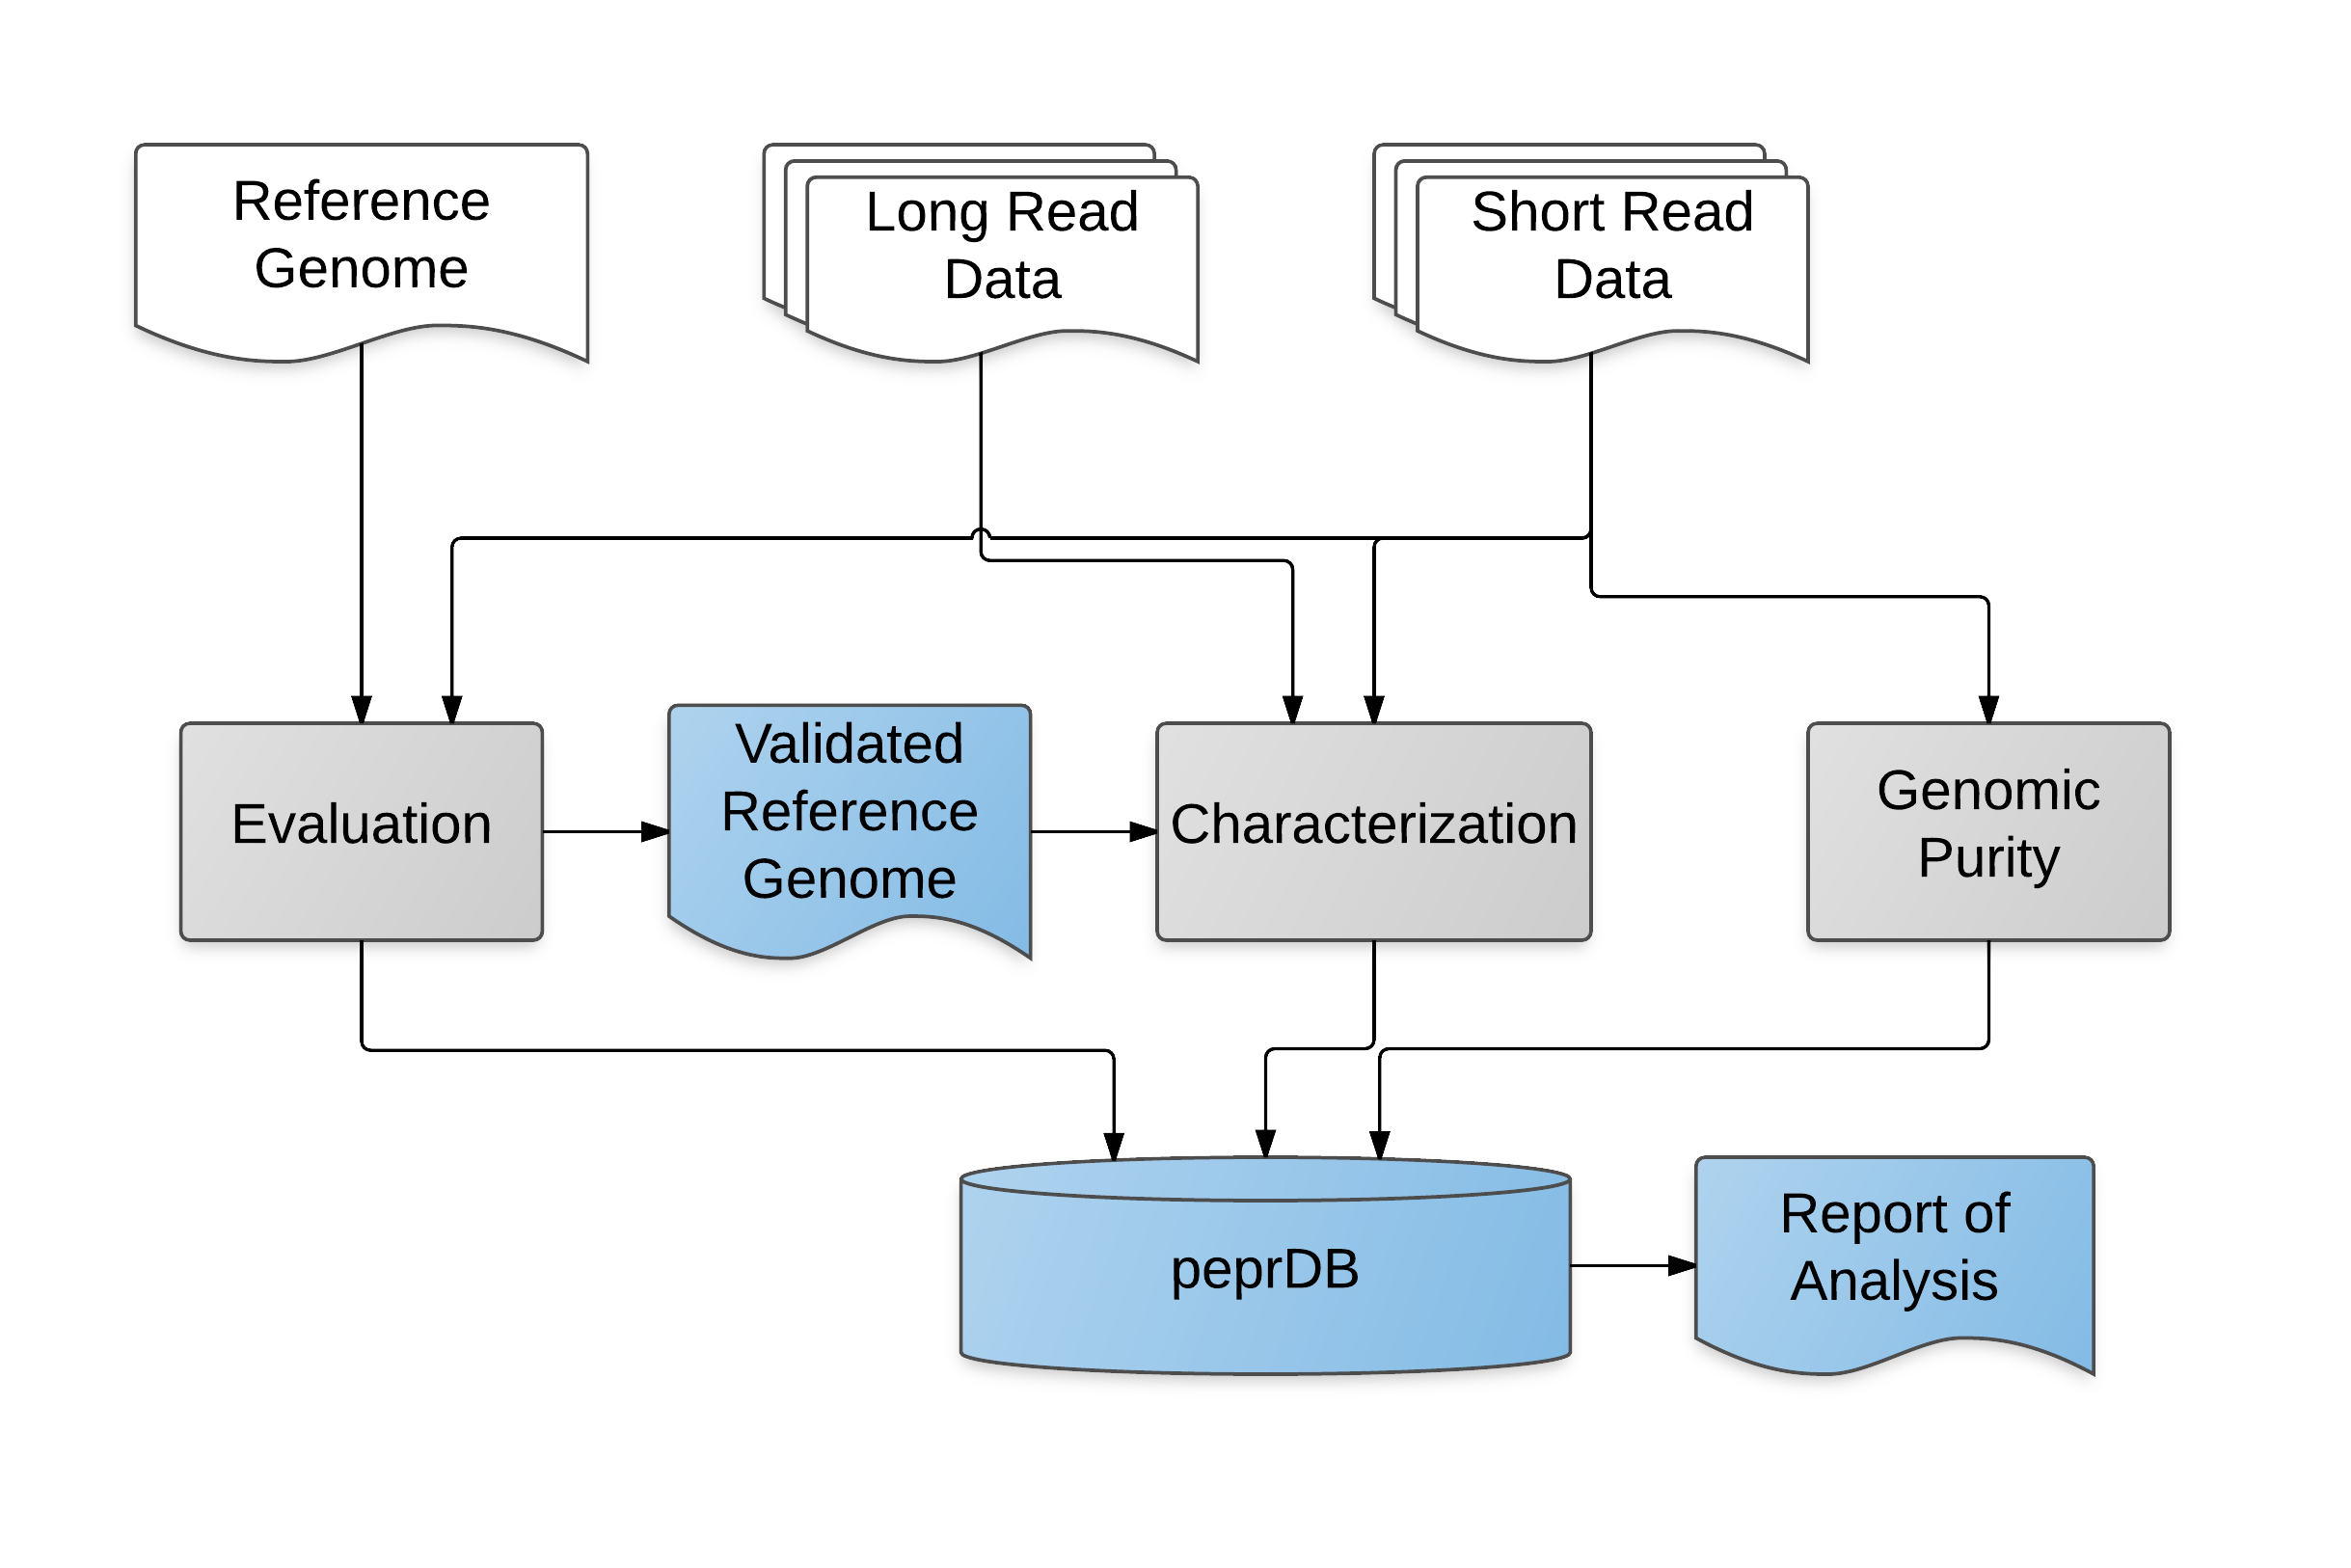
\includegraphics[width=\textwidth]{pepr-workflow.png}
\label{fig:workflowFig}
\caption{PEPR workflow. White objects are pipeline inputs, grey objects are the three pipeline components, light blue objects are the pipeline products.}
\end{figure}

A software package, \texttt{peprr}, was developed for the statistical computing language R \cite{R2015} to compile the output from the genome evaluation, characterization, and genomic purity pipelines . The compiled data was formated into a series of data tables within a SQLite, \texttt{peprDB}, database to facilitate downstream analysis \cite{wickham2014tidy}.  The package includes functions to generate a number of summary tables and figures, including those in this publication.

\subsection{Genome Evaluation Pipeline}
\label{method:2}
The Genome Evaluation Pipeline, is the first step in the PEPR workflow, and is used to reduce errors in the user provided genome assembly prior to characterization. The \texttt{evaluation} pipeline consists of three steps.  Illumina sequencing data are retrieved from the Genbank Sequence Read Archive (SRA) using the sratoolkit \texttt{fastq-dump} command (\url{http://ncbi.github.io/sra-tools/}). Next, sequencing reads are mapped to the reference genome using BWA mem algorithm \cite{Li2013c}. Finally, Pilon is used to evaluate and polish the reference assembly \cite{Walker2014}. The corrected reference genome is then used as input for the Genome Characterization Pipeline.

\subsection{Genome Characterization Pipeline}
\label{method:3}
The Genome Characterization Pipeline uses replicate sequence dataset from multiple sequencing platforms to characterize the corrected reference genome produced by the Genome Evaluation Pipeline at the individual base level. Illumina data are aligned to the reference genome using the same methods as the \texttt{evaluation} pipeline. IonTorrent PGM data using the TMAP algorithm \cite{Homer}. Additionally, if Pacific Biosciences (PacBio) sequencing data is used to generate the input reference assembly.  The PacBio sequencing data is mapped to the reference genome using the BWA mem algorithm \cite{Li2013c} and  Next the sequence alignment files are processed prior to downstream analysis by marking duplicates with Picard's MarkDuplicates command (\url{http://broadinstitute.github.io/picard}) and realigning reads mapping to regions with insertions or deleltion using the GenomeAnalysisToolKit \cite{McKenna2010, DePristo12011}. After refining the alignment files, base level analysis is performed using the short read sequencing data.  For each platform a VCF (variant call format) file with a number of summary statistics is generated using SAMtools mpileup \cite{Li2009}. A base purity metric is calculated from the resulting VCF files. The base purity metric is the number of bases in reads aligned to a genome position that are in agreement with the reference base divided by the total number of reads supporting the alternate base called by SAMtools at that genome position. Homogeneity analysis, a measure of genomic content similarity between vials of the reference material, is performed by first generating a pileup file using SAMtools mpileup for each dataset then performing pairwise tumor-normal variant calling using VarScan \cite{Koboldt2009}. In this work, VarScan looks specifically for differences between vials in the proportion of reads containing variants. A standard Benjamini-Hochberg procedure was used to assess the power of the homogeneity analysis (Supplemental Material, \url{https://github.com/DanSBS/NGSPower}).  Additionally, a number of summary statistics are calculated for the sequencing datasets using Picard's Collect Multiple Metrics (\url{http://broadinstitute.github.io/picard}).  

\subsection{Genome Purity Pipeline}
\label{method:4}
THE Genomic Purity Pipeline assesses the purity of the genomic material, in terms of the presence of DNA from sources other than the expected genus was assessed using the metagenomic taxonomic read classification algorithm PathoScope 2.0 \cite{Hong2014}.  This method uses an expectation maximization algorithm where the sequence data are first mapped to a database comprised of all sequence data in the Genbank nt database (. Then, through an iterative process PathoScope re-assigns ambiguously mapped reads to a taxonomic group based on the proportion of reads mapped unambiguously to individual taxonomic groups in the database. Using short read sequencing data as input PathoScope 2.0 first filters and trims low quality reads (PathoQC), followed by mapping reads to a reference database (PathoMap - a wrapper for bowtie2 \cite{Langmead2012}), then the expectation-maximization algorithm (PathoID) is used for the taxonomic classification.  The annotated Genbank nt database provided by the PathoScope developers was used as the reference database (\url{ftp://pathoscope.bumc.bu.edu/data/nt_ti.fa.gz}). 

\subsection{Candidate Reference Material \textit{S. aureus} Sequencing Data}
Sequencing data and the reference assembly for the NIST candidate reference material \textit{S. aureus} was used to demonstrate how PEPR is used to characterize a genomic material.  A \textit{de novo} genome assembly from Pacific Biosciences (PacBio) long read sequencing data was used as input for PEPR.  Prior to being used as input the assembly was validated using optical mapping data.  Eight replicate vials of the candidate reference material was sequened on the Illumina MiSeq and Ion Torrent PGM sequencing platforms (Supplemental Methods).

\section{Results}
The output from the analysis of the \textit{S. aureus} candidate reference material using PEPR is presented below. The results provide examples of the type of information, summary figures, and tables that can be generated with PEPR.

\subsection{Sequencing Data Summary Statistics}
Summary statistics were calculated for the number of reads, mapped read length, insert size for paired-end datasets as well as coverage for \textit{S. aureus} datasets (Table \ref{Table:seqTable}). The MiSeq sequencing run had an average of  1.7 million paired-end reads per library with a median read length of  232 bp,  whereas the PGM sequencing run produced 0.2 million reads per library on average with a median read length of 232 bp.  The higher throughput and paired-end reads resulted in a higher per-library coverage for MiSeq compared to PGM (251X vs. 36X).  The three PacBio datasets are technical sequencing replicates (SMRT cells) from the same sequencing library, with a median subread length 10436bp and 302X total coverage. Between the three platforms a total coverage of 4611X was obtained.


% latex table generated in R 3.2.2 by xtable 1.7-4 package
% Wed Sep 30 19:53:33 2015
\begin{table}[ht]
\centering
\begin{tabular}{llrrrrrr}
  \hline
Acc. & Plat & Vial & Lib. & Reads & Length (bp) & Insert (bp) & Cov. \\ 
  \hline
SRR1979039 & miseq & 0 & 1 & 3305082 & 230 & 257 & 247 \\ 
  SRR1979040 & miseq & 0 & 2 & 3732088 & 216 & 233 & 263 \\ 
  SRR1979041 & miseq & 1 & 1 & 3973320 & 218 & 242 & 279 \\ 
  SRR1979042 & miseq & 1 & 2 & 3941040 & 223 & 247 & 285 \\ 
  SRR1979043 & miseq & 2 & 1 & 3442554 & 234 & 268 & 261 \\ 
  SRR1979070 & miseq & 2 & 2 & 3226726 & 232 & 268 & 240 \\ 
  SRR1979044 & miseq & 3 & 1 & 3025028 & 233 & 264 & 229 \\ 
  SRR1979045 & miseq & 3 & 2 & 4796382 & 200 & 210 & 303 \\ 
  SRR1979046 & miseq & 4 & 1 & 3338456 & 239 & 278 & 260 \\ 
  SRR1979047 & miseq & 4 & 2 & 2995090 & 237 & 277 & 231 \\ 
  SRR1979048 & miseq & 5 & 1 & 3495384 & 225 & 255 & 255 \\ 
  SRR1979049 & miseq & 5 & 2 & 3116128 & 241 & 281 & 244 \\ 
  SRR1979050 & miseq & 6 & 1 & 3129282 & 237 & 271 & 240 \\ 
  SRR1979060 & miseq & 6 & 2 & 2976312 & 242 & 280 & 233 \\ 
  SRR1979064 & miseq & 7 & 1 & 2630544 & 241 & 283 & 204 \\ 
  SRR1979065 & miseq & 7 & 2 & 3416580 & 225 & 248 & 247 \\ 
  SRR2002412 & pgm & 0 & 1 & 556903 & 231 &  & 42 \\ 
  SRR2002413 & pgm & 1 & 1 & 530117 & 224 &  & 38 \\ 
  SRR2002414 & pgm & 2 & 1 & 437527 & 231 &  & 33 \\ 
  SRR2002415 & pgm & 3 & 1 & 552692 & 232 &  & 42 \\ 
  SRR2002416 & pgm & 4 & 1 & 498479 & 232 &  & 37 \\ 
  SRR2002418 & pgm & 5 & 1 & 390070 & 235 &  & 30 \\ 
  SRR2002419 & pgm & 6 & 1 & 426196 & 232 &  & 32 \\ 
  SRR2002420 & pgm & 7 & 1 & 439119 & 238 &  & 34 \\ 
  SRR2056302 & pacbio & 9 & 1 & 163475 & 10510 &  & 108 \\ 
  SRR2056306 & pacbio & 9 & 2 & 163471 & 10436 &  & 103 \\ 
  SRR2056310 & pacbio & 9 & 3 & 163474 & 9863 &  & 91 \\ 
   \hline
\end{tabular}
\caption{Summary of sequencing datasets.  Acc. - Sequence read archive (SRA) database accessions. Plat. - sequencing platform, miseq: Illumina MiSeq, pgm: Ion Torrent PGM, pacbio: Pacific Biosciences RSII. Lib. - library replicate number for miseq and pgm, smartcell replicate for pacbio. Reads - number of sequencing reads in the dataset. Length - median read length in base pairs.  Insert - median insert size in base pairs for paired end reads.  Cov. - median sequence coverage across the genome.} 
\label{Table:seqTable}
\end{table}


\subsection{Genome Evaluation}
The first step in PEPR is the Genome Evaluation Pipeline.  Short read sequencing data is used to identify and correct errors in the user-provided reference genome, in this case the validated PacBio assembly. Running Pilon using the MiSeq data did not identify any assembly or base call errors. 

\subsection{Base Level Purity}



A base purity metric was used to evaluate the degree to which the sequencing data supports the reference base call.  We compared purity metric values between two orthogonal sequencing methods, MiSeq and PGM, for all positions in the genome (Fig. \ref{fig:purityScatterFig}). Positions with purity metric values greater than 99 \% were categorized as high purity and less than 99 \% low purity. Out of 2909968 positions in the genome 2864925 positions had purity values greater than 99 \% for both short read sequencing platforms (Table \ref{Table:purityTable}).  Further, 2909853 and 2909965 positions had purity values greater than 99 \% and 97 \%, respectively, for one of the two platforms.  Only 115 positions had a purity values less than 99 \% for both platforms, and no positions had a purity value less than 95 \% for both platforms. The positions with low purity for MiSeq were non-uniformly distributed whereas positions with low purity for PGM were uniformly distributed (Fig. \ref{fig:purityPositionFig}).  


% latex table generated in R 3.2.2 by xtable 1.7-4 package
% Wed Sep 30 19:53:35 2015
\begin{table}[ht]
\centering
\begin{tabular}{lrr}
  \hline
  & PGM-High & PGM-Low \\ 
  \hline
MiSeq-High & 2864925 & 44534 \\ 
  MiSeq-Low & 394 & 115 \\ 
   \hline
\end{tabular}
\caption{Number of genome positions with high and low purity, positions purity metric values higher and lower than 0.99 respectively, for the Illumina MiSeq and Ion Torrent PGM sequencing platforms.} 
\label{Table:purityTable}
\end{table}



\begin{knitrout}
\definecolor{shadecolor}{rgb}{0.969, 0.969, 0.969}\color{fgcolor}\begin{figure}

{\centering \includegraphics[width=\maxwidth]{figure/purityScatterFig-1} 

}

\caption[Comparison of base purity values for PGM and MiSeq]{Comparison of base purity values for PGM and MiSeq. Positions are colored based of high and low purity values for the two sequencing platforms, MiSeq - Illumina MiSeq and PGM - Ion Torrent PGM. A purity value of 0.99 was used to differentiate between high and low purity positions. Positions with high purity for both platforms were excluded from the figure.}\label{fig:purityScatterFig}
\end{figure}


\end{knitrout}


\begin{knitrout}
\definecolor{shadecolor}{rgb}{0.969, 0.969, 0.969}\color{fgcolor}\begin{figure}

{\centering 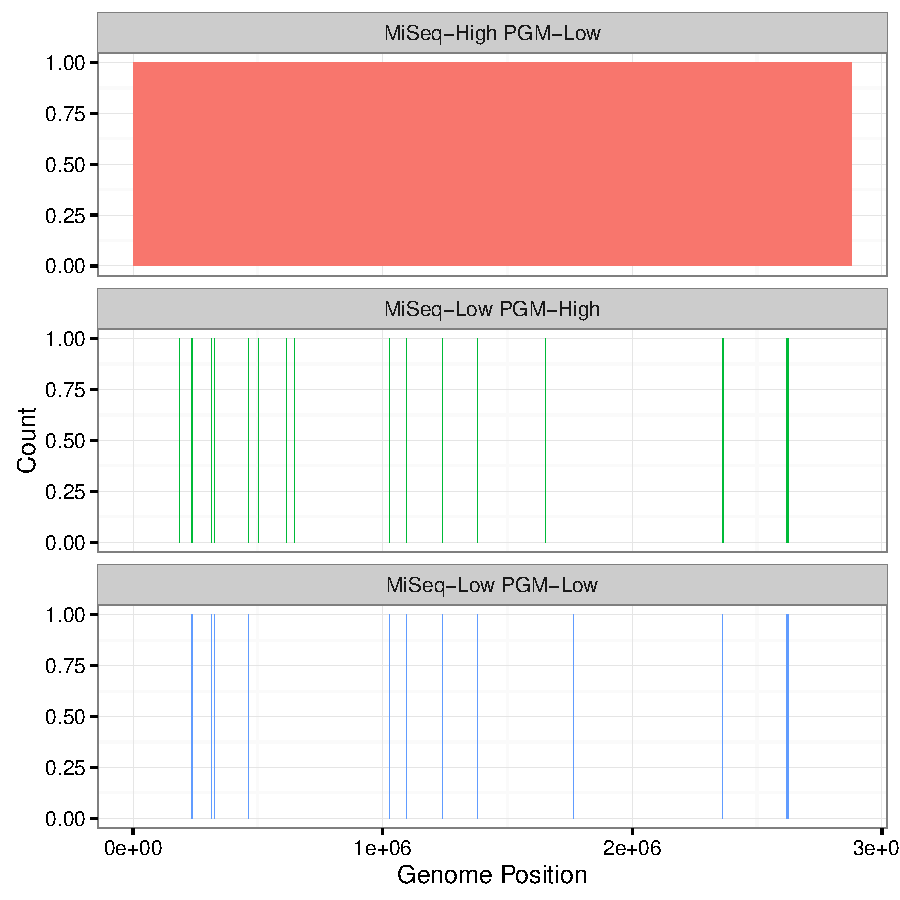
\includegraphics[width=\maxwidth]{figure/purityPositionFig-1} 

}

\caption[Distribution of genome positions by purity group]{Distribution of genome positions by purity group. Bases with high and low purity and purity values greater than and less than 0.99 respectively for the two platforms, MiSeq - Illumina MiSeq and PGM - Ion Torrent PGM.  Positions with high purity for both platforms were excluded from the figure.}\label{fig:purityPositionFig}
\end{figure}


\end{knitrout}


\subsubsection{Base Level Homogeneity}
The genomic material homogeneity was assessed through pairwise statistical analysis of the replicate MiSeq datasets using the VarScan somatic variant caller \cite{Koboldt2009}.  The pairwise variant analysis failed to identify any statistically significant base level differences among the replicates (Table \ref{Table:homogeneityTable}).


% latex table generated in R 3.2.2 by xtable 1.7-4 package
% Wed Sep 30 19:53:37 2015
\begin{table}[ht]
\centering
\begin{tabular}{rrrrr}
  \hline
Position & Proportion of Pairs & Median Frequency & Minimum P-value & N Significant \\ 
  \hline
244332 & 0.01 & 21.31 & 0.51 & 0.00 \\ 
  2615986 & 0.03 & 20.48 & 0.45 & 0.00 \\ 
  2616058 & 0.08 & 25.29 & 0.15 & 0.00 \\ 
  2619808 & 0.01 & 20.78 & 0.61 & 0.00 \\ 
  2619886 & 0.01 & 21.54 & 0.50 & 0.00 \\ 
   \hline
\end{tabular}
\caption{Pairwise variant analysis results. Position is the position in the genome where differences in variant frequency for a least one of the 16 pairwise comparisons were reported. Proportion of pairs is the fraction of the pairwise comparisons between the 16 Illumina MiSeq datasets where a difference in the variant frequency was reported by VarScan. Median frequency is the median variant frequency for the datasets were a difference in the variant frequency was reported. Minimum P-value is the lowest p-value reported by VarScan for all pairwise dataset comparisons where a difference in variant frequency was reported. N Significant is the number of datasets where a reported difference was statistically significant at the genome position.} 
\label{Table:homogeneityTable}
\end{table}



\subsection{Genomic Purity Pipeline}
Short read sequencing data was used to identify the proportion of DNA in the material from an organism other than the material genus, in this case \textit{Staphylococcus}, using PathoScope 2.0 \cite{Hong2014} . Based on analysis of the MiSeq and PGM sequencing data, the reference material has minimal if any genomic contaminants (Fig. \ref{fig:contamCountsFig}), with a maximum of 0.0039 \% reads in any dataset classified as not belonging to the genus \textit{Staphylococcus}. The most abundant contaminant was \textit{Escherichia coli} (Fig. \ref{fig:contamTaxaFig}).  


\begin{knitrout}
\definecolor{shadecolor}{rgb}{0.969, 0.969, 0.969}\color{fgcolor}\begin{figure}

{\centering \includegraphics[width=\maxwidth]{figure/contamCountsFig-1} 

}

\caption[Proportion of reads from contaminant DNA]{Proportion of reads from contaminant DNA. Reads categorized as genomic contaminants as classified by PathoScope as not belonging to the genus \textit{Staphylococcus}.}\label{fig:contamCountsFig}
\end{figure}


\end{knitrout}


\begin{knitrout}
\definecolor{shadecolor}{rgb}{0.969, 0.969, 0.969}\color{fgcolor}\begin{figure}

{\centering 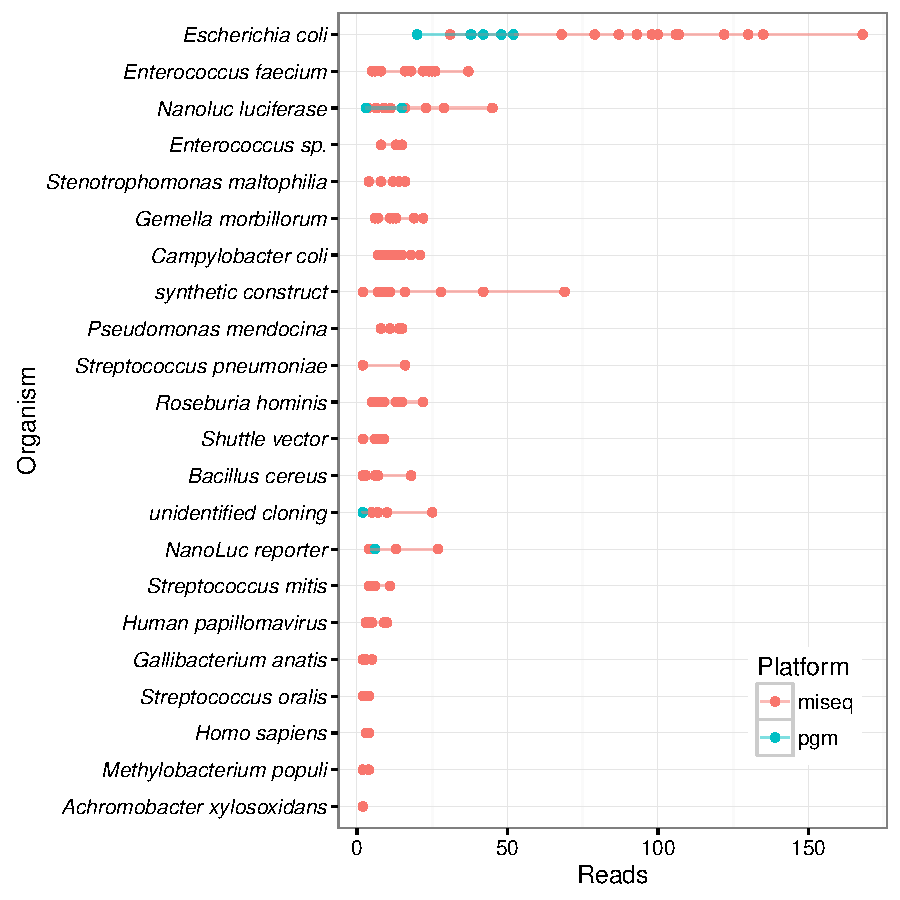
\includegraphics[width=\maxwidth]{figure/contamTaxaFig-1} 

}

\caption[Breakdown of contaminants by organism]{Breakdown of contaminants by organism.}\label{fig:contamTaxaFig}
\end{figure}


\end{knitrout}


\section{Discussion}
\subsection{PEPR}
Pipelines for Evaluating Prokaryotic References (PEPR) is designed to use biological and technical replicate sequencing data from orthogonal sequencing platforms to characterize the genome of a microbial material.  There are two primary reasons for using replicate sequencing datasets one is to test for homogeneity within the batch of DNA being characterized the second is to minimize the impact of library specific biases. The resulting characterized genome is suitable for use in evaluating and benchmarking whole genome sequencing methods. PEPR consists of three pipelines: genome evaluation, genome characterization, and genomic purity assessment.

The PEPR Genome Evaluation Pipeline provides an automated method for evaluating and refining a reference genome sequence. User's provide a high quality reference genome as input to the pipeline. Pilon was chosen for the genome evaluation step as it not only assesses the accuracy of the genome but also corrects errors in the assembly.  Other methods are available for evaluating reference genomes, e.g. amosValidate \cite{Phillippy2008} and ALE \cite{Clark2013}, however these methods only assess assembly accuracy and do not correct missassemblies. The resulting reference assembly represents a consensus genome for the population of cells used to generate the material being characterized.  The genome evaluation pipeline does not attempt to identify or characterize low frequency structural variants within the material or vial-to-vial variability of the reference genome. The reference genome, once validated, and if nessessary refined by the Genome Evaluation Pipeline, is used as input for the Genome Characterization Pipeline. 

The Genome Characterization Pipeline calculates base level statistics using replicate sequencing data from orthogonal measurement methods.  Additionally, the Genome Characterization Pipeline generates summary statistics for the sequencing datasets used in the material characterization procedure as well as long read data if it was used to generate the reference assembly, if applicable.  The results from the Genome Evaluation and Characterization pipeline are loaded into peprDB, a SQLite database. Loading the data into a SQLite database makes it easier to perform additional analyses of the material characterization and evaluation results.

\subsubsection{Process for using PEPR}
If another lab wishes to characterize a new reference or quality control material, they could follow this process:
\begin{enumerate}
    \item Ideally, the user should generate a large batch of material and aliquot it to reduce inhomogeneity.
    \item Identify a high-quality genome assembly. If a good reference assembly does not exist for the sample, then long-read sequencing like PacBio may be required to generate an assembly, and ideally mapping technologies would be used to validate the assembly.
    \item Short-read whole genome sequencing, preferably from two orthogonal sequencing technologies, should be generated from multiple vials of the material, ideally 2 technical replicate libraries from at least six randomly selected vials.
    \item PEPR can then be run to assess base-level purity and homogeneity, genomic contaminants, and mis-assemblies.
The methods presented in this work provide a straightforward pipeline that can be used by any laboratory to characterize new reference materials or in-house quality controls.
\end{enumerate}

\subsection{PEPR Application: Characterization of Candidate RM 8376 using PEPR}
\subsubsection{Preparation of Reference Assembly}
PEPR requires a high quality reference assembly for input, in this work, a closed candidate reference genome was assembled from long read data generate using the Pacific Biosciences RSII platform. Optical mapping technologies and large insert mate-pair library preparation methods, including Illumina's TruSeq Synthetic Long-Reads \cite{McCoy2014}, represent orthogonal methods that can also be used to identify large misassemblies for validating reference assemblies for use in PEPR. To validate the \textit{S. aureus} reference genome, whole genome mapping data generated with the OpGen optical mapping technology, was used to validate the genome assembly. The long DNA fragments (average size \textgreater 200Mb) allow for the evaluation of large misassemblies (\textless 3 kb) that are not easily identified using standard short read sequencing data \cite{Mendelowitz2014}. In this work, after the initial assembly was validated for no large misassemblies, the reference assembly was characterized using PEPR. 

\subsubsection{Sequencing Dataset Summary}
The PEPR database (peprDB) includes a number of summary statistics for the sequencing datasets processed.  For sequencing datasets used to characterize the NIST candidate reference material RM8376, throughput and read lengths were as expected based on the library prep and sequencing methods used excluding the PGM datasets. For PGM the 400 bp sequencing and library preparation methods, median read lengths of 232 bp. The shorter read length is potentially due to the low GC content, which is known to challenge current sequencing technologies \cite{Quail2012}.  

\subsubsection{Base Level Purity}
The ratio of sequencing reads supporting the reference and alternative base call was used to assess the purity of a genome position or base in the material as a whole. Through comparison of the base purity for two orthogonal sequencing methods we identified genome positions with low purity values due to platform specific systematic sequencing errors. The reference base is identified using a third orthogonal sequencing method (Pacific Biosciences RSII), which only chooses the dominant base and does not identify small impurities. Thus, a low purity (below 50 \%) for one of the two short read sequencing platforms and a high purity value for the other means that two technologies (one short read and one long read) agree that the dominant base is the reference base. It is also important to acknowledge that even if the two short read sequencing platforms indicate an impurity, they are potentially susceptible to the same unknown bias. The sequencing technologies used to characterize the material are still maturing and an incomplete understanding of platform specific biases limits our ability to provide a confidence value for the base calls. 

A number of base level metrics, such as strand bias, are calculated as part of the PEPR Genome Characterization Pipeline and are included in the pipeline results database. These metrics can be used to differentiate positions with low purity due to measurement error and those due to biological variability. Use of additional metrics and algorithms developed for the identification of low frequency variants, such as loFreq \cite{Wilm2012}, could help identify positions with low levels of biological variability, but are not currently implemented in PEPR. 

The PEPR Genome Characterization Pipeline assesses the homogeneity of a material through comparison of purity values between replicate vials.  The homogeneity analysis is performed using the VarScan tumor-normal variant caller \cite{Koboldt2009}.  Only Illumina data was used to assess the homogeneity of the material as the higher coverage increased the statistical power of the test, and replicate libraries provide information regarding the method error rate.  The Ion Torrent dataset did not include replicate libraries for the eight vials sequenced and therefore library specific sequencing errors were confounded with vial to vial variability. No statistically significant variants were identified between all pairwise comparisons indicating that the material is homogeneous. If potential inhomogeneities were found, then the PGM sequencing data could be examined for additional support for the inhomogeneities. Even without replicate libraries for the different vials it is unlikely that any library specific bias will correlate with vial-to-vial variability observed in the Illumina data by chance.

\subsection{Genomic Purity Pipeline}
 The Genomic Purity Pipeline is used to identify DNA within the material that belongs to a genus other than the material genus.  The genus level cutoff was selected based on results from a previous study characterizing the specificity of the PathoScope 2.0 classification algorithm (Olson et al. \textit{in-prep}). Genomic contaminants can be from the culture itself or reagents and materials used to prepare the material or during sequencing \cite{Shrestha2013, Tang2003, Salter2014}.  Contaminants identified by the Genomic Purity Pipeline may not be present in the material. For example reagents used during library preparation may also include contaminants \cite{Tanner1998, Newsome2004, Motley2014, Salter2014}.  Additionally, bioinformatic errors may lead to false positive contaminants, either due to errors in the database or bioinformatic errors by classification algorithm.  Genomic purity analysis of the \textit{S. aureus} material identified a number of candidate contaminants,  the most abundant of which was \textit{E. coli}.  \textit{E. coli} is a well documented contaminant of molecular biology reagents, and not likely a true contaminant \cite{Salter2014}. Lower abundant contaminants maybe bioinformatic errors and not true contaminants. While, contaminants identified by the Genomic Purity Pipeline are most likely from reagents and due to bioinformatic errors, a conservative estimate of the material purity, assuming all contaminants are real, reported by the pipeline. Users will want to take into consideration the limited specificity of the taxonomic classification method. For example if the intended use of the genomic DNA is for use as part of an inclusivity exclusivity pannel, additional genomic purity assessment in addition to the PEPR Genomic Purity Pipeline is required to validate the material.

\section{Conclusions}
PEPR provides a framework for characterizing microbial genomic reference materials, for instance a homogenized batch of DNA from a single prokaryotic strain. The objective in developing PEPR was to provide a reproducible and transparent workflow for the characterization of prokaryotic genomic materials. The pipeline can be used to characterize reference materials as well as in-house quality control materials for which replicate sequencing datasets from multiple platforms are available. The outputs from PEPR include a corrected reference genome assembly, identified genome position with high and low purity based on biological and technical variation, base level homogeneity of the material, as well as the percentage and identity of genus level genomic contaminants. The resulting characterization values are intentionally conservative and without uncertainty or confidence estimates, as sources of bias and error associated with the measurement process are currently not fully understood. As the scientific community's understanding of the measurement process matures new algorithms can be incorporated into the pipeline to increase the quality of material characterization process. The genomic materials characterized using PEPR will not only help increase confidence in measurement methods and assays, but can be used to benchmark and validate sequencing platforms and bioinformatic algorithm improving our understanding of sequencing and data analysis process.


\begin{acknowledgements}
The author’s would like to thank Jenny McDaniel, Lindsay Vang, and David Catoe for performing the MiSeq and PGM sequencing, and Tim Muruvanda for performing the PacBio sequencing. Additionally, we would like to thank Drs. Nancy Lin and Steven Lund for converations and suggestions while developing PEPR and drafting the manuscript. This work was supported by the Department of Homeland Security (DHS) Science and Technology Directorate under the Interagency Agreement HSHQPM-14-X-00078 with NIST and by two interagency agreements with the FDA. Opinions expressed in this paper are the authors’ and do not necessarily reflect the policies and views of the DHS, NIST, or affiliated venues. Certain commercial equipment, instruments, or materials are identified in this paper only to specify the experimental procedure adequately. Such identification is not intended to imply recommendation or endorsement by the NIST, nor is it intended to imply that the materials or equipment identified are necessarily the best available for the purpose.
Official contribution of NIST; not subject to copyrights in USA.
\end{acknowledgements}

\printbibliography

\end{document}
% end of file pepr_pub.tex

